\documentclass[twocolumn,a4j]{jsarticle}
\setlength{\topmargin}{-20.4cm}
\setlength{\oddsidemargin}{-10.4mm}
\setlength{\evensidemargin}{-10.4mm}
\setlength{\textwidth}{18cm}
\setlength{\textheight}{26cm}

\usepackage[top=15truemm,bottom=20truemm,left=20truemm,right=20truemm]{geometry}
\usepackage[latin1]{inputenc}
\usepackage{amsmath}
\usepackage{amsfonts}
\usepackage{amssymb}
\usepackage[dvipdfmx]{graphicx}
\usepackage[hang,small,bf]{caption}
\usepackage[subrefformat=parens]{subcaption}
\usepackage[dvipdfmx]{color}
\usepackage{listings}
\usepackage{listings,jvlisting}
\usepackage{geometry}
\usepackage{framed}
\usepackage[dvipdfmx]{hyperref}
\usepackage{ascmac}
\usepackage{enumerate}
\usepackage{tabularx}
\usepackage{cancel}
\usepackage{scalefnt}
\usepackage{overcite}
\usepackage{otf}
\usepackage{multicol}
\usepackage[geometry]{ifsym}
\usepackage{array}

\renewcommand{\figurename}{Fig.}
\renewcommand{\tablename}{Table }

\lstset{
basicstyle={\ttfamily},
identifierstyle={\small},
commentstyle={\smallitshape},
keywordstyle={\small\bfseries},
ndkeywordstyle={\small},
stringstyle={\small\ttfamily},
frame={tb},
breaklines=true,
columns=[l]{fullflexible},
xrightmargin=0zw,
xleftmargin=3zw,
numberstyle={\scriptsize},
stepnumber=1,
numbersep=1zw,
lineskip=-0.5ex
}

% キャプション後ろのダブルコロンを消す
\makeatletter
\long\def\@makecaption#1#2{%
  \vskip\abovecaptionskip
  \iftdir\sbox\@tempboxa{#1\hskip1zw#2}%
    \else\sbox\@tempboxa{#1 #2}%
  \fi
  \ifdim \wd\@tempboxa >\hsize
    \iftdir #1\hskip1zw#2\relax\par
      \else #1 #2\relax\par\fi
  \else
    \global \@minipagefalse
    \hbox to\hsize{\hfil\box\@tempboxa\hfil}%
  \fi
  \vskip\belowcaptionskip}
\makeatother

% タイトル
\makeatletter
\def\@maketitle
{
\begin{center}
{\LARGE \@title \par}
\end{center}
\begin{flushright}
{\large \@date 報告書 No.36}\\
{\large M2 \@author}
\end{flushright}
\par\vskip 1.5em
}
\makeatother

\author{来代 勝胤}
\title{令和4年度 10月 第3週 報告書}
\date{2022/10/17}

\begin{document}
\columnseprule=0.1mm
\maketitle

\section*{報告内容}
\begin{enumerate}[1.]
  \item 解析アルゴリズムの修正
  \item マッチングアルゴリズムの検討
  \item 来週の予定
\end{enumerate}

\section{解析アルゴリズムの修正}
クラスタの追跡アルゴリズムについて,
プログラムを見直し,その修正を行った.
ここで,これまで使用していたのクラスタの平均値を用いたニアレストマッチングと
今回修正を行ったクラスタの近似直線を用いたラインマッチングの性能に比較について
三角翼後流の解析結果を用いて示す.\\

\subsection{右翼後流 (翼端から後方 0mm地点,800 枚)}
はじめに,これまでも扱ってきた右翼後流の解析結果を示す.
また,今回は$y-z$平面の速度ベクトル場に加えて主流方向速度および渦度を表示している.
これらの結果をみると,$y-z$平面内の速度ベクトルについて,
Nearest matching アルゴリズムに比べて
Line matching アルゴリズムの方が,速度が大きく評価されていることがわかる.

\begin{figure}[htbp]
  \subsubsection*{$\blacksquare$ 主流方向速度}
  \centering
  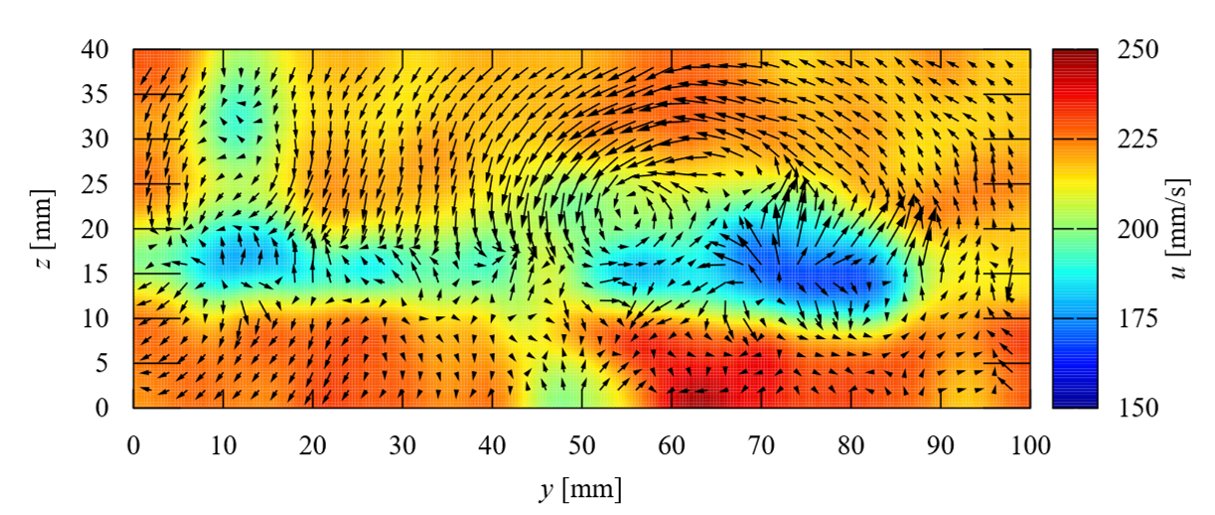
\includegraphics[keepaspectratio, width=80mm]{../images/vel_n_R.png}
  \caption{Right : Nearest matching}
  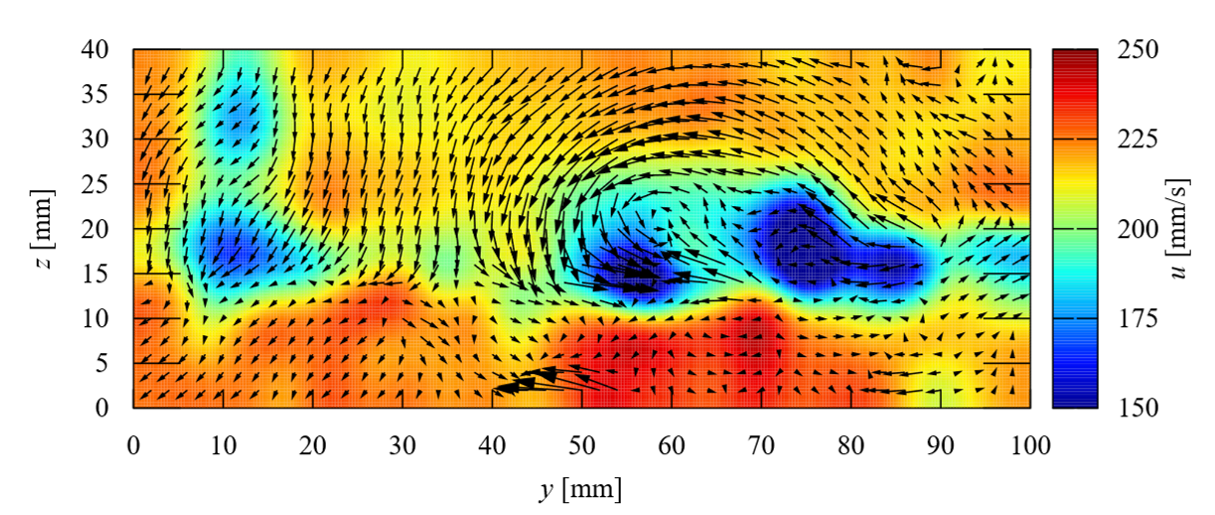
\includegraphics[keepaspectratio, width=80mm]{../images/vel_l_R.png}
  \caption{Right : Line matching}
\end{figure}

\newpage
また,主流方向速度について,Line matching アルゴリズムでは,
局所的な速度を捉えられていることがわかる.
これは,時刻経過によって発生する粒子の移動を情報に含めているため,
より妥当なペアの選択が可能になったと考えられる.

\begin{figure}[htbp]
  \subsubsection*{$\blacksquare$ 渦度}
  \centering
  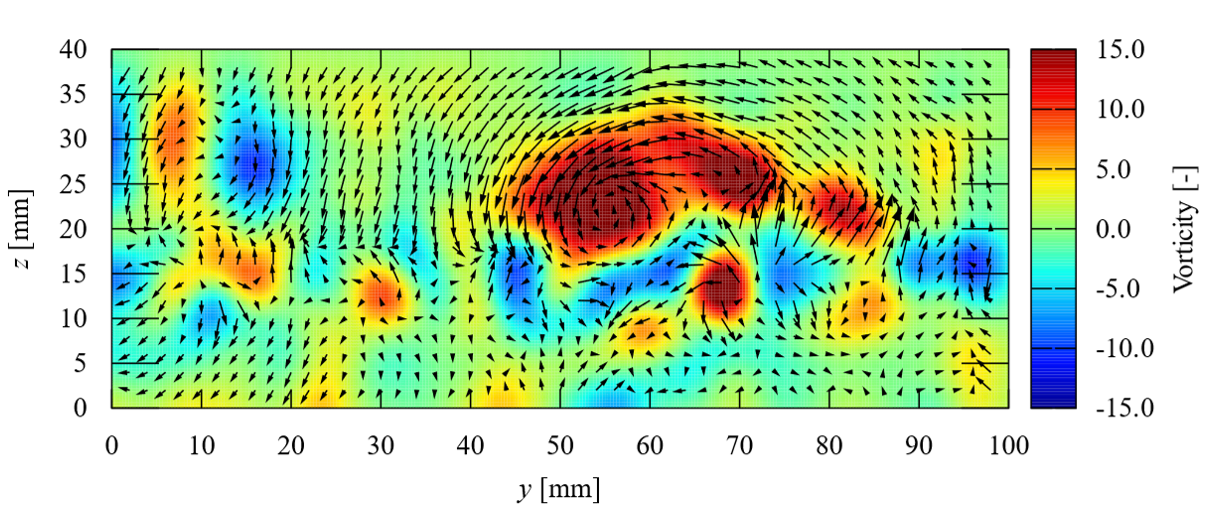
\includegraphics[keepaspectratio, width=80mm]{../images/vor_n_R.png}
  \caption{Right : Nearest matching}
  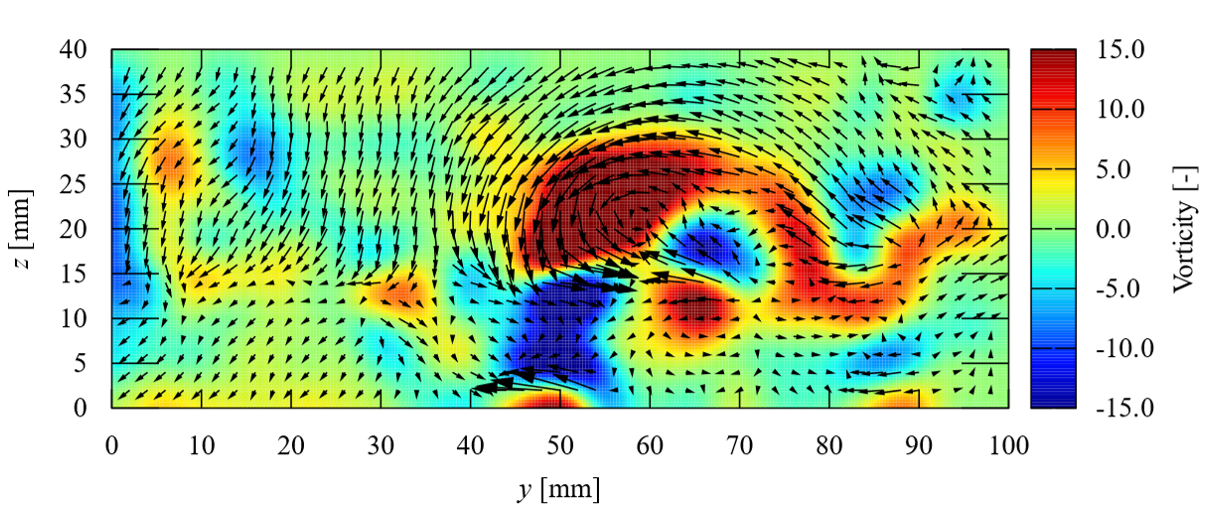
\includegraphics[keepaspectratio, width=80mm]{../images/vor_l_R.png}
  \caption{Right : Line matching}
\end{figure}

\subsection{左翼後流 (翼端から後方 50mm地点,800枚)}
\begin{figure}[htbp]
  \subsubsection*{$\blacksquare$ 主流方向速度}
  \centering
  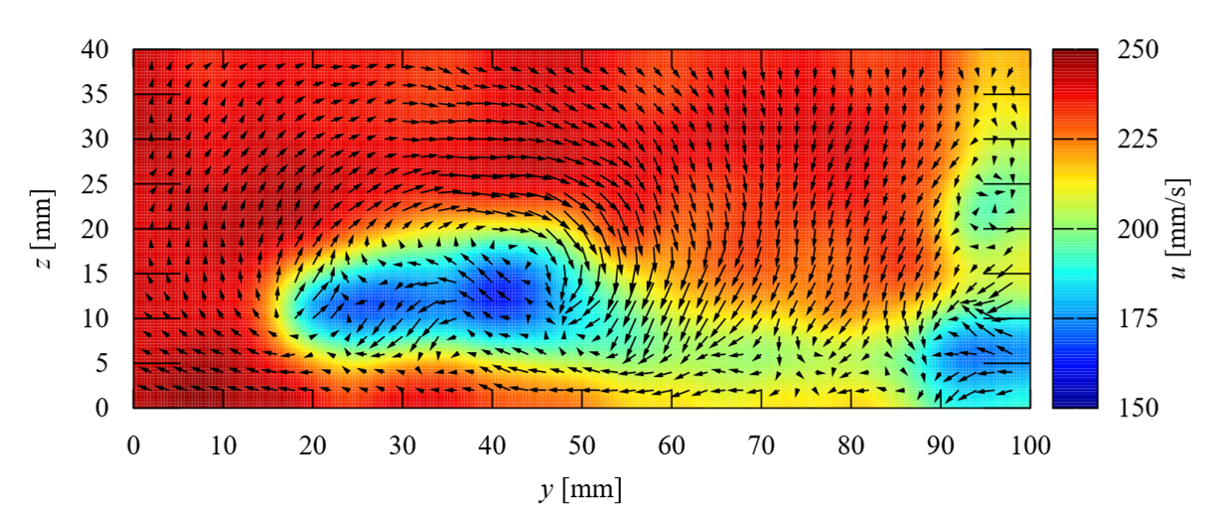
\includegraphics[keepaspectratio, width=80mm]{../images/vel_n_L.png}
  \caption{Left : Nearest matching}
  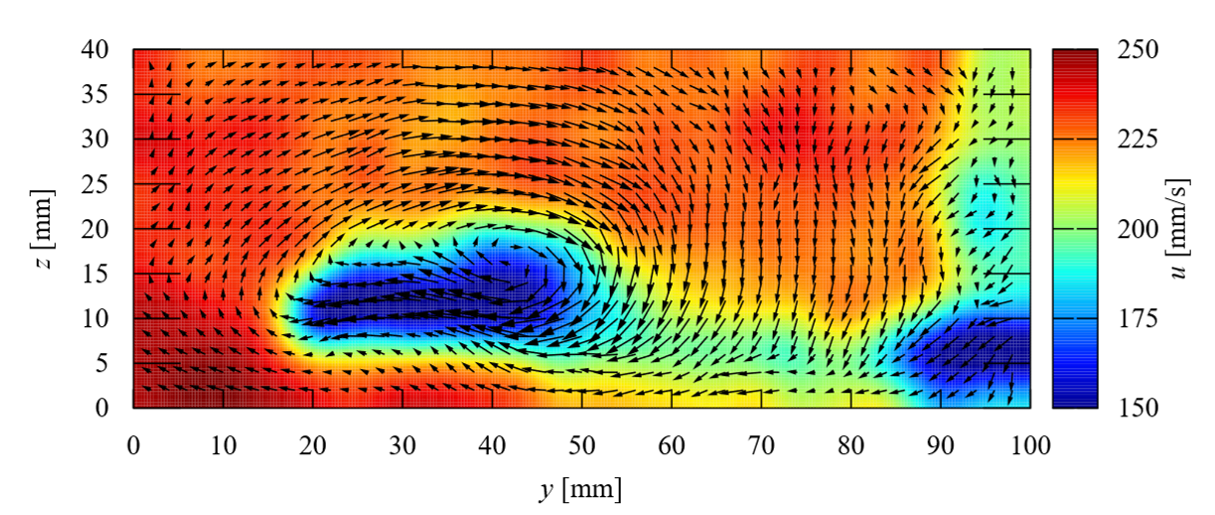
\includegraphics[keepaspectratio, width=80mm]{../images/vel_l_L.png}
  \caption{Left : Line matching}
\end{figure}

\newpage
\section{マッチングアルゴリズムの検討}
\subsection{単位の統一}
これまでのマッチングアルゴリズムでは,
単位の異なる $n\;[\rm{\#}], y\;[\rm{pixel}], z\;[\rm{pixel}]$ の
3つの変数を用いて,マッチングの指標を計算していた.
そこで,以下のような式を用いて単位を統一する.

\begin{eqnarray*}
  x' &=& n \times \frac{U}{f} \\
  y' &=& C_a\;y\\
  z' &=& C_b\;z\\
  U &:& 主流速度 [\rm{mm/s}]\\
  f &:& フレームレート [\rm{fps}]\\
  C_a &:& 係数 [\rm{mm/pixel}]\\
  C_b &:& 係数 [\rm{mm/pixel}]\\
\end{eqnarray*}

また,校正画像を用いて,$C_a, C_b$ を求める.
校正画像内から2点の代表点を定め,画像内の距離を計算する.
\begin{figure}[htbp]
  \centering
  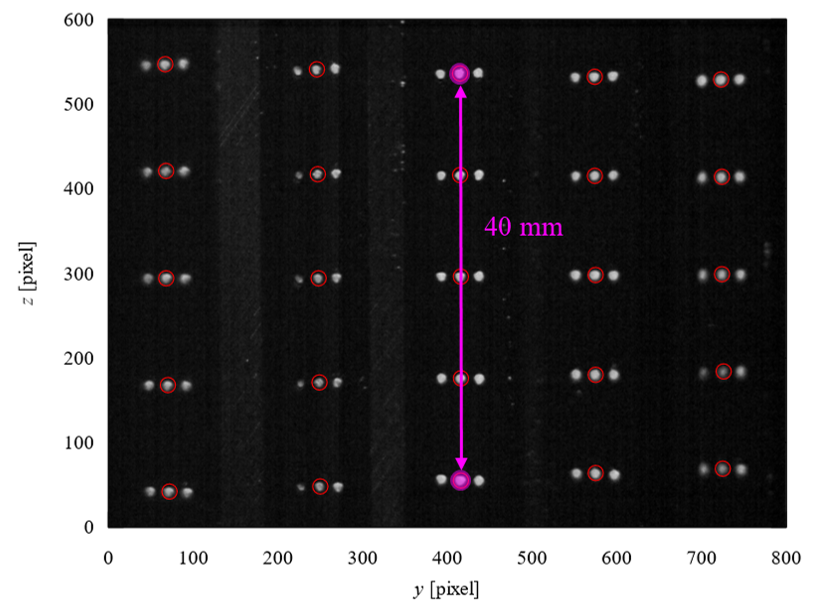
\includegraphics[keepaspectratio, width=85mm]{../images/calibration.png}
  \caption{Calibration of the unit}
\end{figure}


\section{来週の予定}
\begin{itemize}
  \item マッチングアルゴリズムの検討 (続き)
\end{itemize}

\end{document}